\documentclass{article}
\usepackage[utf8]{inputenc}
\usepackage{fullpage}
\usepackage[T1]{fontenc}
\usepackage{amsmath,amsthm,amssymb,amsfonts, mathtools, physics}
\usepackage{enumitem, verbatim, float}
\usepackage[brazil]{babel}
\usepackage{enumitem}

\title{2\textsuperscript{o} Exercício Escolar de Sistemas de Controle - 2019.1}
\author{Turma de Sistemas de Controle de 2019.1}
\date{}

\begin{document}

\maketitle

\section{Questão 1}

    Resolva o seguinte problema de programação não linear:

    
    $$ Max F(x_{1}, x_{2}) = - \left( x_{1} - \frac{5}{2} \right)^2 - \frac{1}{2} \left( x_{2}  + 4 \right)^2 $$
    
    sujeito a: 
    
    $$ g_{1}(x_{1}, x_{2}) =  \left( x_{1} - 2 \right)^2 +  \left( x_{2}  - 2 \right)^2 \leq 1 $$
    
    $$ g_{2}(x_{1}, x_{2}) =  \left( x_{1} - 3 \right)^2 +  \left( x_{2}  - 2 \right)^2 \leq 1 $$
    
    $$ x_{1} \geq 0 , \: \: x_{2} \geq 0  $$
    
    \subsection{Resposta:}
    
        Inicialmente, verifica-se o ponto de gradiente nulo de $F(x_{1}, x_{2})$  sem restrições. Isto é, $\nabla F = 0$. 
        
        Assim, temos: 
        
        $$ \left\{
                \begin{array}{ll}
                  \frac{\partial F}{\partial x_{1}} = 0 \vspace{0.3cm} \\
                  
                  \frac{\partial F}{\partial x_{2}} = 0
                \end{array}
              \right.
            \quad  \implies \quad 
            \left\{
                \begin{array}{ll}
                  x_{1} = 2,5 \vspace{0.1cm} \\
                  
                  x_{2} = -4
                \end{array}
              \right.
         $$
         
     \vspace{0.6cm}
     
    Em seguida, verifica-se o domínio das restrições $g_{1}$ e $g_{2}$. 
    
    Observa-se as curvas de nível de $g_{1}$, $g_{2}$ e $\nabla F$ na Figura \ref{dominio}.
    
        \begin{figure}[H]
            \centering
            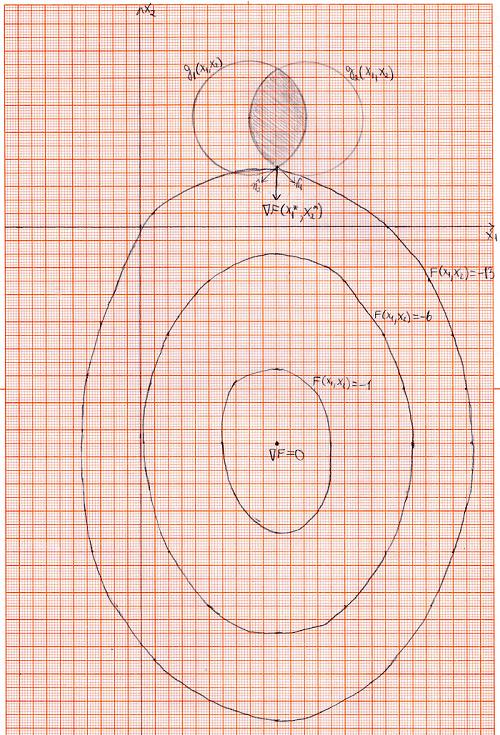
\includegraphics[scale=1]{q1.png}
            \caption{Domínio das restrições e $\nabla F$.}
            \label{dominio}
        \end{figure}
    
        
    Percebe-se que o ponto de máximo de $F(x_{1}, x_{2})$ está fora do domínio de de $g_{1} \cap g_{2} $. Assim, a solução ótima encontra-se na fronteira do domínio das restrições.
    
    A partir da análise geométrica, percebe-se que o ponto de interseção inferior entre as curvas $g_{1}$ e $g_{2}$ é um forte candidato à ponto de máximo. Isto é, o ponto $(x_{1}$, $x_{2}) = (2.5; 1,134 )$ 
    
    Além disso, percebe-se que:
            
             $$ \left\{
                \begin{array}{ll}
                  \pdv[2]{F}{x_{1}} = -2 < 0 \vspace{0.3cm} \\
                  
                  \pdv[2]{F}{x_{2}} = -1 < 0 \vspace{0.3cm} \\
                \end{array}
              \right.
            $$
    
    Isso implica que a função $F(x_{1}, x_{2})$ é côncava.
    Da mesma maneira verifica-se que as restrições $g_{i}(x_{1}, x_{2})$ são convexas.
    
    Dessa forma, podemos verificar as condições de Karush-Kuhn-Tucker no ponto desejado e verificar se o mesmo é ponto de máximo.
    
    Para isso, escreve-se o Lagrangeano:
    
    $$ L(x_{1}, x_{2}, y_{1}, y_{2} ) = - \left( x_{1} - \frac{5}{2} \right)^2 - \frac{1}{2} \left( x_{2}  + 4 \right)^2 + y_{1}\left( 1- \left( x_{1} - 2 \right)^2 -  \left( x_{2}  - 2 \right)^2 \right) + y_{2} \left( 1- \left( x_{1} - 3 \right)^2 -  \left( x_{2}  - 2 \right)^2 \right) $$
    
    Daí, temos as condições de Karush-Kuhn-Tucker:
    
        $$ \left\{
                \begin{array}{l}
                  \frac{\partial L}{\partial x_{1}} = -2\left( x_{1}  - \frac{5}{2} \right) -2y_{1}(x_{1} - 2) -2y_{2}(x_{1} - 3) \leq 0  \vspace{0.3cm} \\
                  
                  \frac{\partial L}{\partial x_{2}} = -\left( x_{2}  + 4 \right) -2y_{1}(x_{2} - 2) -2y_{2}(x_{2} - 2) \leq 0  \vspace{0.3cm} \\
                  
                  x_{1}\left( -2\left( x_{1}  - \frac{5}{2} \right) -2y_{1}(x_{1} - 2) -2y_{2}(x_{1} - 3) \right) = 0  \vspace{0.3cm} \\
                  
                  x_{2}\left(  -\left( x_{2}  + 4 \right) -2y_{1}(x_{2} - 2) -2y_{2}(x_{2} - 2) \right) = 0 \vspace{0.3cm}  \\
                  
                  y_{1}\left(  1- \left( x_{1} - 2 \right)^2 -  \left( x_{2}  - 2 \right)^2   \right) = 0 \vspace{0.3cm}  \\
                  
                  y_{2} \left( 1- \left( x_{1} - 3 \right)^2 -  \left( x_{2}  - 2 \right)^2 \right)  = 0 \vspace{0.3cm}  \\
                  
                   x_{1} \geq 0 , \: \: x_{2} \geq 0, \:\: y_{1} \geq 0 , \: \: y_{2} \geq 0
                  
                \end{array}
              \right. $$
              
       \vspace{0.8 cm}       
       
       Aplica-se o ponto candidato a máximo nas condições 3 e 4. Tem-se que: 
        
            $$ \left\{
                \begin{array}{l}
                  
                  2.5\left( -2\left( 2.5  - \frac{5}{2} \right) -2y_{1}(2.5 - 2) -2y_{2}(2.5 - 3) \right) = 0 \vspace{0.3cm} \\
                  
                  1,134\left(  -\left( 1,134  + 4 \right) -2y_{1}(1,134 - 2) -2y_{2}(1,134 - 2) \right) = 0 \vspace{0.3cm}  \\
                  
                \end{array}
              \right. 
              \quad  \implies \quad
              \left\{
                \begin{array}{l}
                  
                   -y_{1} + y_{2} = 0  \vspace{0.3cm} \\
                  
                  -5,134 + 1,732 y_{1} + 1,732 y_{2} = 0 \vspace{0.3cm}  \\
                  
                \end{array}
              \right.
              $$
              
        Isso resulta em $y_{1} =  y_{2} = 1,48$. 
        
        A partir dos valores de  $y_{1}$ e $y_{2}$ encontrados e dos valores de $x_{1}$ e $x_{2}$ do ponto candidato, verifica-se que todas as condições de Karush-Kuhn-Tucker são satisfeitas.
        
        Logo, sabendo que $F(x_{1}, x_{2})$ é côncava, as restrições $g_{i}(x_{1}, x_{2})$ são convexas e que as condições de  Karush-Kuhn-Tucker são todas satisfeitas no ponto $(x_{1}$, $x_{2}) = (2.5; 1,134 )$, pode-se afirmar que o máximo da função $F(x_{1}, x_{2})$ sujeita as condições $g_{1}$ e $g_{2}$ é $F(2,5 , \: 1,134) = -13, 178$
        

        
   
\newpage
\section{Questão 2}
    
    Resolva o seguinte problema de programação não linear:

    
    $$ Max F(x_{1}, x_{2}) =  x_{1} ^2 - x_{2}^2 $$
    
    sujeito a: 
    
    $$ g_{1}(x_{1}, x_{2}) =    x_{1}  - \frac{16}{25} \left( x_{2}  - 1 \right)^2 -4 \leq 0 $$
    
    $$ g_{2}(x_{1}, x_{2}) =    x_{1}  -  \left( x_{2}  - 2 \right)^2 -4 \leq 0 $$
    
    $$ g_{3}(x_{1}, x_{2}) =   - x_{1}  + 8x_{2}  -28 \leq 0 $$
    
    $$ x_{1} \geq 0 , \: \: x_{2} \geq 0  $$
    
\subsection{Resposta}

     Inicialmente, verifica-se os pontos críticos de $F(x_{1}, x_{2})$  sem restrições. Isto é, $\nabla F = 0$. 
        
        Assim, temos: 
        
        $$ \left\{
                \begin{array}{ll}
                  \frac{\partial F}{\partial x_{1}} = 0 \vspace{0.3cm} \\
                  
                  \frac{\partial F}{\partial x_{2}} = 0
                \end{array}
              \right.
            \quad  \implies \quad 
            \left\{
                \begin{array}{ll}
                  x_{1} = 0 \vspace{0.1cm} \\
                  
                  x_{2} = 0
                \end{array}
              \right.
         $$
         
     \vspace{0.6cm}
     
    Em seguida, verifica-se o domínio das restrições $g_{1}$, $g_{2}$ e $g_{3}$. 
    
    Observa-se o domínio das restrições e $\nabla F$ na Figura \ref{g1-g2-g3-F-r}.
    
        \begin{figure}[H]
            \centering
            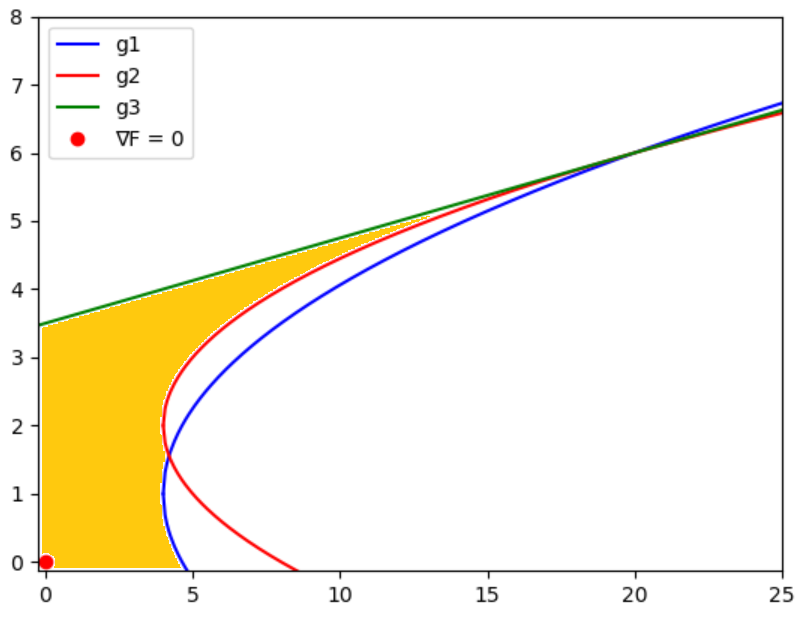
\includegraphics[scale=1]{g1-g2-g3-F-r.png}
            \caption{Domínio das restrições e $\nabla F = 0$.}
            \label{g1-g2-g3-F-r}
        \end{figure}
    
    Nota-se que uma das diferenças essenciais entre esse problema e o da 1\textsuperscript{a} questão é que o ponto $\nabla F = 0$ está no domínio das restrições. Outra diferença crucial é que esse ponto não é um ponto de máximo, mas sim um ponto de sela. Isso se deve ao fato de que a função a ser maximizada é um paraboloide hiperbólico.
    
    Uma consequência importante dessa geometria é que a função $F(x_{1}, x_{2})$ não é côncava. Assim, as condições de Karush-Kuhn-Tucker tornam-se condições necessárias, mas não suficientes. Dessa forma, necessita-se verificar a natureza da função a ser otimizada. 
    
    A partir de $F(x_{1}, x_{2}) = x_{1}^2 - x_{2}^2$, percebe-se que, no ponto de máximo, deve-se encontrar um valor que maximiza $x_{1}$ e minimiza $x_{2}$. Desse modo, o ponto de máximo de $F(x_{1}, x_{2})$ se encontra na extremidade direita da região do domínio das restrições. 
    
    Sendo assim, toma-se o ponto de encontro entre $g_{1}$ e o eixo $x_{2} = 0$ ($x_{1}=4,64$ e $x_{2} = 0$) como um possível candidato a ponto de máximo. Ao analisar o domínio das restrições, com auxílio dos gráficos da Figura \ref{g1-g2-g3-F-r}, percebe-se que existe um conjunto de curvas na extremidade direita do domínio das restrições em que os pontos contidos nessas curvas possuem a coordenada $x_{1}$ menor do que $4,64$ e coordenada $x_{2}$ maior de que $0$. Logo, $F(x_{1}, x_{2})= x_{1}^2 - x_{2}^2$ avaliada em qualquer um desses pontos é menor do que $F(x_{1}, x_{2})$ avaliada no atual candidato a máximo. 
    
    Ainda assim, existe um um intervalo que necessita uma investigação aprofundada. Esse é o intervalo da extremidade do domínio que coincide com a restrição $g_2$ a partir do ponto $(x_{1}, x_{2})= (4,64, \: 2,8)$ até se encontrar com as restrições $g_1$ e $g_3$ ($x_{1}=20$ e $x_{2} = 6$). Nesse segmento, percebe-se que os valores de $x_{1}$ crescem mais rapidamente que os valores de $x_2$. Por conseguinte, $F(x_{1}, x_{2})$ é crescente a medida que se ''caminha'' na curva em direção ao ponto na extrema direita. 
    
    Portanto, tem-se dois ponto candidatos a máximo. O ponto $(x_{1}, x_{2})= (4,64, \: 0)$ e o ponto $(x_{1}, x_{2})= (20, \: 6)$. 
    
    Analisa-se as codições de Karush-Kuhn-Tucker nos pontos.
    
    Para isso, escreve-se o Lagrangeano:
    
    $$ L(x_{1}, x_{2}, y_{1}, y_{2} ) =  x_{1} ^2 - x_{2}^2 + 
    y_{1}\left(4 - x_{1}  + \frac{16}{25} \left( x_{2}  - 1 \right)^2  \right)   +
    y_{2} \left(4 - x_{1}  +  \left( x_{2}  - 2 \right)^2 \right)+
    y_{3} \left(28 + x_{1}  -  8x_{2} \right) $$
    
    Daí, tem-se as condições de Karush-Kuhn-Tucker:
    
        $$ \left\{
                \begin{array}{l}
                  \frac{\partial L}{\partial x_{1}} = 2x_{1} -y_{1} -y_{2}+y_{3} \leq 0  \vspace{0.3cm} \\
                  
                  \frac{\partial L}{\partial x_{2}} = -2x_{2} +\frac{32}{25}y_{1}(x_{2} - 1) +2y_{2}(x_{2} - 2)-8y_{3} \leq 0  \vspace{0.3cm} \\
                  
                  x_{1}\left( 2x_{1} -y_{1} -y_{2}+y_{3} \right) = 0  \vspace{0.3cm} \\
                  
                  x_{2}\left(  -2x_{2} +\frac{32}{25}y_{1}(x_{2} - 1) +2y_{2}(x_{2} - 2)-8y_{3} \right) = 0 \vspace{0.3cm}  \\
                  
                  y_{1}\left(4 - x_{1}  + \frac{16}{25} \left( x_{2}  - 1 \right)^2  \right) = 0 \vspace{0.3cm}  \\
                  
                  y_{2} \left(4 - x_{1}  +  \left( x_{2}  - 2 \right)^2 \right)  = 0 \vspace{0.3cm}  \\
                  
                  y_{3} \left(28 + x_{1}  -  8x_{2} \right)  = 0 \vspace{0.3cm}  \\
                  
                   x_{1} \geq 0 , \: \: x_{2} \geq 0, \:\: y_{1} \geq 0 , \: \: y_{2} \geq 0 , \: \: y_{3} \geq 0
                  
                \end{array}
              \right. $$
              
       \vspace{0.8 cm}        
       
       Aplica-se o ponto candidato  a máximo, $(x_{1}, x_{2})= (4,64, \: 0)$ nas condições 6 e 7. Tem-se que, $y_{2} = y_{3} = 0$. A partir disso, a condição 3 fica: 
       
       $$  x_{1}\left( 2x_{1} -y_{1} -0+0 \right) = 0 $$
              
        Isso resulta em $y_{1}= 2x_{1} = 9,28$.
        
        Isso implica que esse ponto é válido como candidato, mas ainda necessita-se verificar o outro ponto. 
        
        Aplica-se o ponto candidato  a máximo, $(x_{1}, x_{2})= (20, \: 6)$ nas condições 3 e 4. Tem-se que:
        
             $$ \left\{
                \begin{array}{l}
                  
                  20\left( 2\times20 -y_{1} -y_{2}+y_{3} \right) = 0 \vspace{0.3cm} \\
                  
                   6\left(  -2\times6 +\frac{32}{25}y_{1}(6 - 1) +2y_{2}(6 - 2)-8y_{3} \right) = 0 \vspace{0.3cm}  \\
                  
                \end{array}
              \right. 
              \quad  \implies \quad
              \left\{
                \begin{array}{l}
                  
                    y_{1} = 192,5  \vspace{0.3cm} \\
                  
                    y_{2} \geq 0 \vspace{0.3cm}  \\
                  
                    y_{3} = 0,5(2 y_{2} + 305) = 0 \vspace{0.3cm}  \\
                \end{array}
              \right.
              $$
    
    Nota-se que as condições de KKT também são satisfeitas e este pondo também é válido como candidato. 
    
    Portanto, resta avaliar $F(x_{1}, x_{2})$ nos pontos. Tem-se que $F(4,64, \:  0) = 21,53$ e $F(20, \:  6) = 364$. 
    
    Finalmente, afirma-se que o ponto que maximiza $F(x_{1}, x_{2})= x_{1}^2 - x_{2}^2$ sujeito as restrições exigidas é o ponto $(x_{1}, x_{2})= (20, \: 6)$ e $F_{Max} = 364$.


\newpage
\section{Questão 3}

    A Babel S.A. acha que sua rede interna de comunicações telefônicas está falhando em satisfazer às necessidades na hora de pico por causa da capacidade limitada de transmissão e pediu conselho a um consultor de comunicações, Cantu Chammas. Duas estações originam chamadas e três estações recebem as chamadas; mais de uma chamada pode ser enviada ou recebida por qualquer estação. As chamadas são transmitidas através de enlaces e dois nós de comutação. A Figura \ref{arq} ilustra a situação.
    
    \begin{figure}[H]
            \centering
            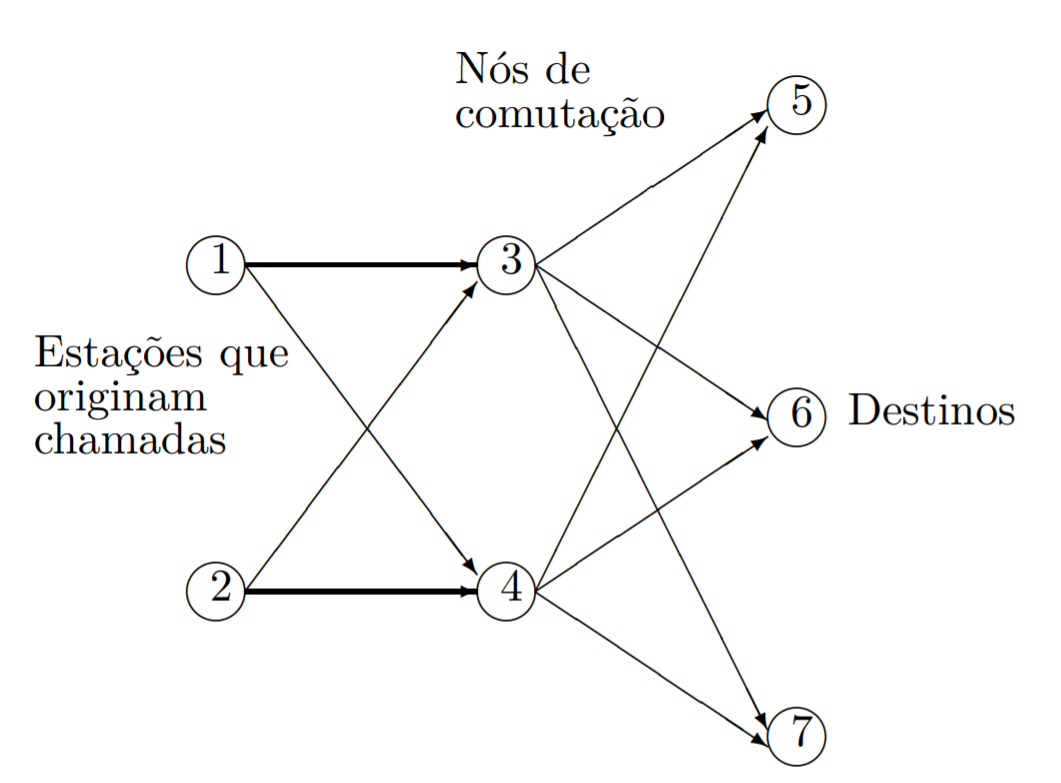
\includegraphics[scale=0.35]{figura.png}
            \caption{Arquitetura do sistema de comunicações.}
            \label{arq}
        \end{figure}
    
    O problema de decisão com que se defronta o Sr. Chammas é aumentar a capacidade de transmissão da rede de maneira econômica. Aumentar a capacidade para enfrentar todas as necessidades nas horas de pico pode ser caro demais, mas alguma melhoria no serviço é necessária.
    
    Seja \(a_{ij}\) as necessidades diárias nas horas de pico de mensagens originadas na Estação \textit{i} e destinadas à Estação \textit{j}, onde \(i = 1\) e \(2\) e \(j = 5, 6\) e \(7\). Seja \(C_{kj}\) a capacidade atual de transmissão de enlace entre o Nó de Comutação \textit{k} e o destino \textit{j}, onde \(k = 3\) e \(4\), e \(j = 5, 6\) e \(7\). Seja \(S_{k}\) a capacidade de transmissão atual para mensagens fluindo através do Nó de Comutação \textit{k}. Defina:
    
   \(x_{ijk} \equiv\) o número de chamadas originadas na Estação \textit{i},
destinadas à Estação \textit{j} e passando através do Nó de Comutação \textit{k}.

\(c_{jk} \equiv\) nova capacidade de transmissão ao longo do enlace entre o Nó de Comutação \textit{k} e o destino \textit{j}.

\(s_{k} \equiv\) nova capacidade de transmissão através do Nó de Comutação \textit{k}.

As restrições a serem satisfeitas são:

   \begin{enumerate}[label=(\roman*)]
       \item O número total de chamadas de cada estação de origem a cada destino não pode exceder as necessidades nas horas de pico para tais chamadas.
       \item O número total de chamadas passando ao longo do enlace entre um nó de comutação e um destino não pode exceder a correspondente capacidade de transmissão do enlace.
       \item O número total de chamadas passando através de qualquer nó de comutação não pode exceder a correspondente capacidade de transmissão.
       \item As novas capacidades de enlaces e nós devem ser pelo menos tão grandes quanto as atuais.
   \end{enumerate}
   
  A exigência de nível de serviço é especificada como segue. A rota das chamadas deve satisfazer à restrição de que a relação do número \textit{total} de chamadas que são realmente transmitidas pela soma de todas as necessidades nas horas de pico deve ser pelo menos \textit{f} (onde \(f < 1\)).
  
  O custo de aumentar de uma unidade a capacidade de transmissão de enlace entre o Nó de Comutação \textit{k} e o Destino \textit{j} é \(d_{kj}\), e o de aumentar de uma unidade a capacidade de transmissão do Nó de Comutação \textit{k} em uma unidade é \(d_{k}\).
  
  Mostre como uma formulação de programação linear pode ser usada para achar um plano de mínimo-custo para aumentar as capacidades de enlaces e nós, respeitadas as restrições mencionadas acima.

\subsection{Resposta:}

    Deseja-se encontrar um plano de mínimo-custo para aumentar as capacidades de enlaces e nós; isto é, encontrar quantas unidades de capacidades de enlaces e nós devem ser aumentadas de forma a minimizar seu custo. Dessa forma, as variáveis do problema podem ser definidas como:

\(U_{kj} \equiv\) Número de unidades aumentadas da capacidade de transmissão de enlace entre o Nó de Comutação \textit{k} e o Destino \textit{j}.

\(U_{k} \equiv\) Número de unidades aumentadas da capacidade de transmissão do Nó de Comutação \textit{k}.

De maneira que a capacidade atual de transmissão de enlace entre o Nó de Comutação e o destino, adicionada ao número de unidades aumentadas dessa capacidade de transmissão, seja igual a nova capacidade de transmissão ao longo do enlace entre o Nó de Comutação e o destino. Portanto:
\begin{equation*}
   C_{kj} + U_{kj} = c_{kj} 
\end{equation*}

$$ \left\{
                \begin{array}{l}
                  C_{35} + U_{35} = c_{35}  \vspace{0.3cm} \\
                  
                  C_{36} + U_{36} = c_{36}  \vspace{0.3cm} \\
                  
                  C_{37} + U_{37} = c_{37}  \vspace{0.3cm} \\
                  
                  C_{45} + U_{45} = c_{45}  \vspace{0.3cm} \\
                  
                  C_{46} + U_{46} = c_{46}  \vspace{0.3cm} \\
                  
                  C_{47} + U_{47} = c_{47} 
                \end{array}
              \right. $$

Analogamente, a capacidade de transmissão atual para mensagens fluindo através do Nó de Comutação, adicionada ao número de unidades aumentadas da capacidade de transmissão do Nó, é igual a nova capacidade de transmissão através do Nó de Comutação:

\begin{equation*}
    S_{k} + U_{k} = s_{k}
\end{equation*}
        $$ \left\{
                \begin{array}{l}
                  S_{3} + U_{3} = s_{3}  \vspace{0.3cm} \\
                  
                  S_{4} + U_{4} = s_{4}
                \end{array}
              \right. $$
              
Quanto às restrições:

(i)  O número total de chamadas de cada estação de
origem a cada destino não pode exceder as necessidades nas horas de pico para tais chamadas.

Para obter o número total de chamadas de cada estação de
origem a cada destino é preciso adicionar, para cada estação de origem e destino, as chamadas que passam por cada um dos nós intermediários:

\begin{equation*}
    \sum_{k=3}^{4}(x_{ijk}) \leq a_{ij} \hspace{0.5cm} \therefore \hspace{0.5cm} x_{ij3} + x_{ij4} \leq a_{ij}
\end{equation*}

        $$ \left\{
                \begin{array}{l}
                  x_{153} + x_{154} \leq a_{15}  \vspace{0.3cm} \\
                  
                  x_{163} + x_{164} \leq a_{16}  \vspace{0.3cm} \\
                  
                  x_{173} + x_{174} \leq a_{17}  \vspace{0.3cm} \\
                  
                  x_{253} + x_{254} \leq a_{25} \vspace{0.3cm}  \\
                  
                  x_{263} + x_{264} \leq a_{26} \vspace{0.3cm}  \\
                  
                  x_{273} + x_{274} \leq a_{27} 
                \end{array}
              \right. $$

(ii)  O número total de chamadas passando ao longo
do enlace entre um nó de comutação e um destino
não pode exceder a correspondente capacidade de
transmissão do enlace.

O número total de chamadas passando ao longo
do enlace entre um nó de comutação e um destino é a soma de todas as chamadas que passam pelo nó de comutação e destino de cada uma das estações de origem:

\begin{equation*}
    \sum_{i=1}^{2}(x_{ijk}) \leq c_{kj} \hspace{0.5cm} \therefore \hspace{0.5cm} x_{1jk} + x_{2jk} \leq c_{kj}
\end{equation*}

        $$ \left\{
                \begin{array}{l}
                  x_{153} + x_{253} \leq c_{35}  \vspace{0.3cm} \\
                  
                  x_{154} + x_{254} \leq c_{45}  \vspace{0.3cm} \\
                  
                  x_{163} + x_{263} \leq c_{36}  \vspace{0.3cm} \\
                  
                  x_{164} + x_{264} \leq c_{46} \vspace{0.3cm}  \\
                  
                  x_{173} + x_{273} \leq c_{37} \vspace{0.3cm}  \\
                  
                  x_{174} + x_{274} \leq c_{47} 
                \end{array}
              \right. $$

(iii) O número total de chamadas passando através de
qualquer nó de comutação não pode exceder a correspondente capacidade de transmissão.

Pode-se obter o número total de chamadas passando através de
qualquer nó realizando o somatório de todas as possíveis estações de origem e de destino de cada nó:

\begin{equation*}
    \sum_{i=1}^{2}\sum_{j=5}^{7}(x_{ijk}) \leq s_{k} \hspace{0.3cm} 
    \therefore \hspace{0.3cm} x_{15k} + x_{16k} + x_{17k} + x_{25k} + x_{26k} + x_{27k} \leq s_{k}
\end{equation*}

        $$ \left\{
                \begin{array}{l}
                  x_{153} + x_{163} + x_{173} + x_{253} + x_{263} + x_{273} \leq s_{3}  \vspace{0.3cm} \\
                  
                  x_{154} + x_{164} + x_{174} + x_{254} + x_{264} + x_{274} \leq s_{4}
                \end{array}
              \right. $$

(iv) As novas capacidades de enlaces e nós devem ser
pelo menos tão grandes quanto as atuais.

Como as variáveis são o número de unidades aumentadas para cada capacidade, esta restrição implica que estas variáveis devem ser maiores ou iguais a zero:

\begin{equation*}
U_{kj} \geq 0 \hspace{0.3cm} ; \hspace{0.3cm} U_{k} \geq 0
\end{equation*}

Quanto à restrição à nível de serviço, a relação do número total de chamadas que são realmente transmitidas pela soma de todas as necessidades nas horas de pico deve ser pelo menos \textit{f}:

\begin{equation*}
    \frac{\sum_{i=1}^{2}\sum_{j=5}^{7}\sum_{k=3}^{4}(x_{ijk})}{\sum_{i=1}^{2}\sum_{j=5}^{7}(a_{ij})} \geq f
\end{equation*}

\begin{equation*}
    \frac{x_{153} + x_{154} + x_{163} + x_{164} + x_{173} + x_{174} + x_{253} + x_{254} + x_{263} + x_{264} + x_{273} + x_{274}}{a_{15} + a_{16} + a_{17} + a_{25} + a_{26} + a_{27}} \geq f
\end{equation*}

O custo \textit{K} para aumentar as capacidades de enlaces e nós é o custo de aumentar cada unidade d as capacidades de transmissão de enlace e nócvezes a quantidade de unidades aumentadas para cada enlace e nó:

\begin{equation*}
    K = \sum_{k=3}^{4}\sum_{j=5}^{7} d_{kj}\cdot U_{kj} + \sum_{k=3}^{4} d_{k}\cdot U_{k}
\end{equation*}

\begin{equation*}
    K = d_{35}\cdot U_{35} + d_{36}\cdot U_{36} + d_{37}\cdot U_{37} + d_{45}\cdot U_{45} + d_{46}\cdot U_{46} + d_{47}\cdot U_{47} + d_{3}\cdot U_{3} + d_{4}\cdot U_{4}
\end{equation*}

Objetiva-se minimizar este custo, isto é, maximizar o negativo do custo:

\begin{equation*}
   Max F = -\sum_{j=5}^{7}\sum_{k=3}^{4} d_{kj}\cdot U_{kj} - \sum_{k=3}^{4} d_{k}\cdot U_{k}
\end{equation*}

\begin{equation*}
   Max F = - d_{35}\cdot U_{35} - d_{36}\cdot U_{36} - d_{37}\cdot U_{37} - d_{45}\cdot U_{45} - d_{46}\cdot U_{46} - d_{47}\cdot U_{47} - d_{3}\cdot U_{3} - d_{4}\cdot U_{4}
\end{equation*}

\newpage
\section{Questão 4}
    Um problema clássico de sistemas de controle é
    aquele de transferir um sistema dinâmico de um estado
    inicial especificado para um estado final especificado em
    tempo mínimo, sendo a força de controle limitada, cotada,
    superiormente e inferiormente. A solução para
    este tipo de problema envolve o princípio do bang-bang,
    pois a força de controle assume apenas o valor máximo
    ou o valor mínimo (ou seja, $u = 1$ ou $u = -1$), o que
    torna a solução muito menos dispendiosa.
    Considere o sistema definido por:
    $$
    \dot{x} =  
    \begin{bmatrix} 0 & 1 \\ 0 & 0 \end{bmatrix}x + 
    \begin{bmatrix} 0 \\ 1 \end{bmatrix}u & \text{ , onde $-1\leq u \leq 1$}
    $$
    Trata-se de levar o sistema de uma condição inicial qualquer
    $(x_{1}(t_{0}), x_{2}(t_{0}))$ até a origem (0, 0), num tempo
    mínimo.
    
    a) Formule o problema de controle ótimo correspondente.
    
    b) Resolva o problema de controle ótimo formulado no item a).
    
    c) Identifique, no plano de fase ($x_{1},x_{2}$), o lugar geométrico dos pontos de condições iniciais onde não será necessário nenhum chaveamento da força de controle para se atingir a origem em tempo mínimo. Esboce as trajetórias no plano de fase e explique.
    
    d) Qual é o número mínimo de chaveamentos necessários para que o sistema evolua de qualquer condição inicial para qualquer condição final em tempo mínimo?
    \subsection{Resposta:}
        \subsubsection{Letra a)}
            O problema do controle ótimo é expresso por:
            
           $$ Max J = \int_{t_{0}}^{t_{1}} I(x,u,t) dt$$
    
            sujeito a: 
    
            $$ \frac{dx}{dt} =  f(x,u,t) $$
    
            Este problema consiste em encontrar uma função de controle ótima (u) que maximize o funcional objetivo (J), respeitando as restrições impostas. Para solucionar tais problemas é utilizado o Princípio do Máximo de Pontryagin.
            
             Para o problema de interesse, temos a seguinte formulação:
    
             $$ Max J = \int_{t_{0}}^{t_{1}} -1 dt$$
    
                sujeito a: 
    
            $$ \frac{dx_{1}}{dt} =  x_{2} $$
            $$ \frac{dx_{2}}{dt} =  u $$
            $$ -1\leq u \leq 1$$
            $$ x_{1}(t_{1}) = 0, x_{2}(t_{1}) = 0$$
        
        \subsubsection{Letra b)}
            Define-se o Hamiltoniano como:
            
            $$ H(x,u,t,y) = I(x,u,t) + y^Tf(x,u,t)$$
            
            Pelo Princípio do Máximo de Pontryagin, a função ótima ($u^*$) é aquela que maximiza o Hamiltoniano satisfazendo as condições:
            
            $$ \left\{
                \begin{array}{ll}
                  \frac{dx_{i}}{dt} = \pdv{H}{y_{i}} \vspace{0.3cm} \\
                  
                  \frac{dy_{i}}{dt} = -\pdv{H}{x_{i}} \\
                \end{array}
              \right.
            $$
            
            No problema de interesse temos:
            $$ H(x,u,t,y) = -1+y_{1}x_{2}+y_{2}u$$
            Assim,
            
            $$ \left\{
                \begin{array}{ll}
                  \frac{dy_{1}}{dt} = -\pdv{H}{x_{1}} = 0 \vspace{0.3cm} \\
                  
                 \frac{dy_{2}}{dt} = -\pdv{H}{x_{2}} = -y_{1}
                \end{array}
              \right.
            \quad  \implies \quad 
            \left\{
                \begin{array}{ll}
                  y_{1} = c_{1} \vspace{0.1cm} \\
                  
                  y_{2} = c_{2}-c_{1}t
                \end{array}
              \right. & \text{, em que $c_{1},c_{2}$ são constantes.}
         $$
         
         Note que o Hamiltoniano é linear com relação a u, portanto seu máximo será nos limites do intervalo de u, portanto:.
         
         \[
            u^*= 
            \begin{cases}
            1 ,& \text{se } y_{2}> 0\\
             -1,              & \text{se } y_{2}<0
            \end{cases}
        \]
        
        
        Ou seja, 
        $$ u^{*}(t) = sinal(c_{2}-c_{1}t)$$
        
        
        \subsubsection{Letra c)}
            Substituindo a força de controle encontrada no item b) na equação do sistema dinâmico, temos:
            $$ \left\{
                \begin{array}{ll}
                  \frac{dx_{1}}{dt} = x_{2} \vspace{0.3cm} \\
                  
                 \frac{dx_{2}}{dt} = \pm 1
                \end{array}
              \right.
            \quad  \implies \quad 
            \frac {dx_{2}}{dx_{1}} = \frac{\pm 1}{x_{2}}
         $$
         
         As trajetórias no plano de fase são descritas pela seguinte equação:
         
         $$ x_{1} = \frac{\pm x_{2}^2}{2} + k \text{  , em que k é uma constante}$$
         
         Note que para cada valor de k existe um par de parábolas simétricas que correspondem a $u = 1$ e $u = -1$, o chaveamento ocorre na interseção entre essas parábolas, porém quando k = 0 as parábolas se intersectam na origem, que é justamente o estado final, portanto não ocorre chaveamento para este caso. 
         É possível observar o lugar geométrico dos pontos de condições iniciais em que não é necessário chaveamento na Figura \ref{plano_fase}.
         
         \begin{figure}[H]
            \centering
            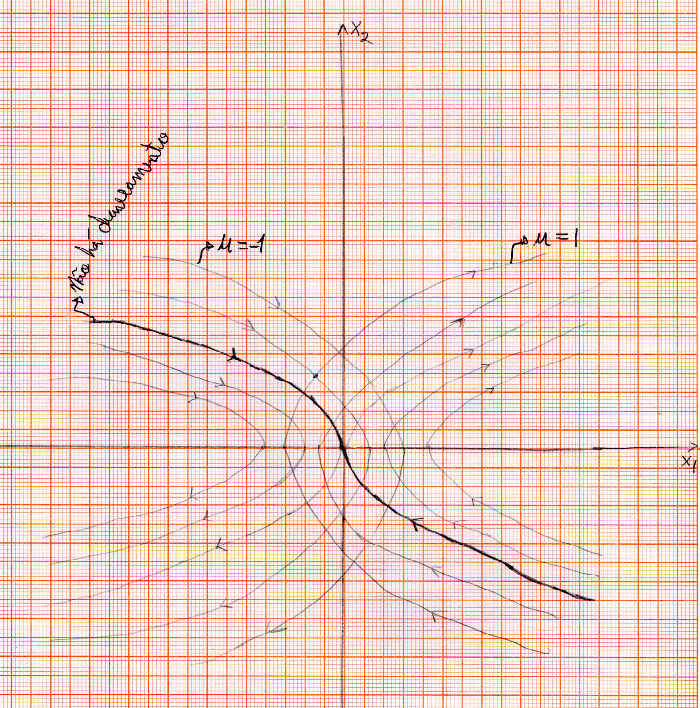
\includegraphics[scale=1]{plano_fase_1.png}
            \caption{Trajetórias no Plano de Fase do sistema dinâmico.}
            \label{plano_fase}
        \end{figure}
         
        \subsubsection{Letra d)}
            A partir da função de controle ótima encontrada no item b) é possível observar que o chaveamento ocorre quando quando $ c_{2}-c_{1}t = 0$. Para qualquer intervalo $[t_{0},t_{1}]$ existe no máximo uma raíz para esta equação. Logo, conclui-se que para o sistema evoluir do estado inicial ao estado final em tempo mínimo é necessário no máximo um chaveamento.
\end{document}
